\Chapter{Automatizálható Webapplikáció Tervezése}

A fejezet célja, hogy a korábban megismert fogalmak és elvárások segítségével, létrehozzunk egy alkalmazás csontvázat aminek az implementálásával egy jól strukturált könnyen karbantartható és fejleszthető megoldást valósíthassunk meg.

További fejlesztések esetén ezen dokumentáció alapján, akár új fejlesztők is betudjanak csatlakozni a megvalósításba.  

\Section{Architektúra felépítése}

\subsection{Több rétegű alkalmazás}
Az MNV ismertetése során felmerült már a Többrétegű alkalmazás architektúra, lényegében véve nem sokban különbözik egymástól a két rendszer struktúrája, csupán további rétegeket vezetünk be, annak érdekében, hogy alkalmazásunkban jobban elkülönítsük a rétegek szerepeit. Ebben a felépítésben viszonylag kötöttebb szabályok mentén kell haladnunk, de az adataink a rétegek közötti átalakítások miatt nagyobb biztonságban vannak.

Hátránya viszont, a kódsorok száma és a fejlesztési idő is jelentősen megnövekedhet az alkalmazásával.

A rendszer tervezett felépítése a \aref{fig:architektura}. ábrán látható, ahol megfigyelhetjük, hogyan halad végig a különböző rétegeken a felhasználói kérés. 

\vskip 0.2in
Az ábrán látható folyamat során a felhasználótól érkező adat feldolgozódik a megjelenítési rétegben, majd az általunk írt Angular applikáció egy JSON objektumot generál és egy HTTP híváson keresztül megszólítja a szerveren futó alkalmazást. 

\begin{figure}[h]
	\centering
	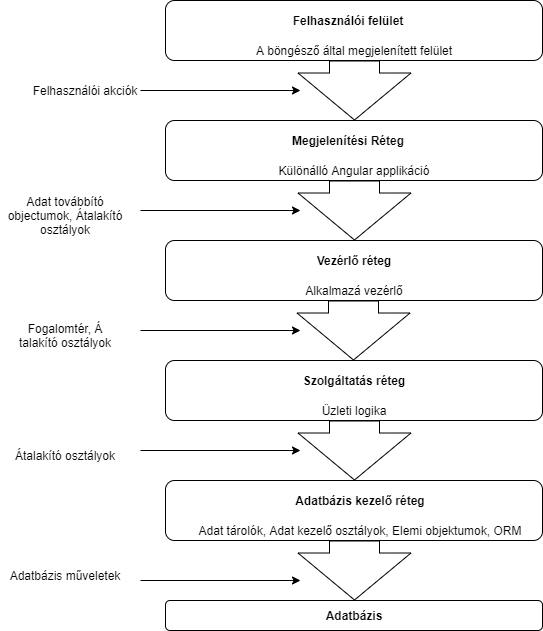
\includegraphics[scale=0.6]{images/applikacio_architektura.png}
	\caption{Többrétegű alkalmazás architektúra.}
	\label{fig:architektura}
\end{figure}

A háttérrendszer által definiált végponton a beérkező JSON kérést egy Adatközvetítő objektummá alakítjuk\footnote{Ennek az objektumtípusnak a fontosságát később kifejtem.}, ezt az objektumot átalakítva átadjuk a szolgáltatási rétegnek. 

Ebben a rétegben feldolgozzuk az adatokat, számításokat végzünk vele, majd a végső formájában átadjuk ismét egy átalakító osztálynak ahol Elemi objektummá alakítjuk.

Az adatkezelő rétegben, hozzáférünk az adatbázis kapcsolatainkhoz így az Elemi értékekből SQL-t létrehozva tudjuk meghívni az adatbázis egyes tábláit, ezzel beszúrni vagy akár lekérdezni adatokat azokból.

\subsection{Megjelenítési réteg}

Az alkalmazásunk itt rendereli ki a felhasználó számára látható és elérhető weboldalt, ez a művelet jól elkülöníthető, akár külön kódbázis és infrastruktúra is tartozhat hozzá, amennyiben nem a már említett JSP technológiát vagy sablon alapú megjelenítést használjuk.
\vskip 0.2in

Az Angulár használata mindenféleképp külön webszerver indítását igényli így érdemes ennek megfelelően különálló logikaként kezelni, akár egy önálló microalkalmazásként is tekinthetünk rá.

A programozási nyelv segítségével képesek vagyunk dinamikusan ellenőrizni a felhasználótól kapott bemeneti értékeket és nem megfelelő adat esetén rögtön jelezni az eltérést, ezzel segítve az elvárt működést.

Fontos, hogy a felhasználói felület letisztult és könnyen használható legyen, ugyanakkor az adatok kezelésében minden esetben a felület igazodik, a szerver oldali logikához. Nem itt definiáljuk az elküldött vagy elvárt JSON üzenetek tartalmát és felépítését. Több fejlesztő esetén a résztvevők közösen egyeznek meg az értékekről és a struktúráról.

\paragraph{Általános felület terv:} A könnyen kezelhetőséget szem előtt tartva a \aref{fig:felület_terv}. látható listanézetes megjelenítést érdemes használni az alkalmazás összes funkciójánál, hogy egyes adatokat megjelenítsünk.

Ennek a nézetnek a segítségével láthatóvá tesszük az elérhető adatokat, azokat az elhelyezett gombok segítségével szerkeszthetjük amik kattintás után az ehhez szükséges űrlaphoz navigálnak. Ezen az oldalon továbbá elérhetőnek kell lennie az elemi műveletekhez szükséges gomboknak mint például törlés, mentés.

\begin{figure}[h]
	\centering
	\includegraphics[scale=0.3]{images/felület.png}
	\caption{Általános felület terv}
	\label{fig:felület_terv}
\end{figure}

\footnote{A jogkörökről és azokhoz tartozó funkciókról a dolgozta későbbi részében lesz szó.}

Az általános felület mintájára a következő típusú felületek megvalósítása szükséges:

\begin{enumerate}
	\item Minden felhasználó számára elérhető.
	\begin{itemize}
		\item Saját adatok megtekintése.
		\item Felhasználható és felhasznált szabadnapok nyomon követése.
		\item Szabadnapok kiírása és módosítása.
	\end{itemize}
	\item Jóváhagyó számára elérhető.
	\begin{itemize}
		\item Vele relációban álló felhasználók szabadnapjainak nyomon követése.
		\item Jóváhagyásra váró kérések listája, azokhoz tartozó műveletek.
	\end{itemize}
	\item Adminisztrátor számára elérhető
	\begin{itemize}
		\item Szabadságolással kapcsolatos konfigurációs oldalak.
		\item Vele relációban álló felhasználók létrehozása, adatainak módosítása.
	\end{itemize}
\end{enumerate}

Továbbá az adminisztrátor és a jóváhagyó számára egy statisztikai összesítéseket megjelenítő oldal, valamint egy éves szabadságolási terv létrehozására és módosítására alkalmas naptár nézettel rendelkező oldal megvalósítására is szükség van.

\subsection{Vezérlő réteg, és Adatközvetítő objektumok}

Az alkalmazásunk szerver oldali megvalósítása a vezérlőrétegnél kezdődik, itt definiálhatjuk a végpontokat amik segítségével kommunikálhatunk a közvetlen felettünk lévő réteggel. Ezek a végpontok URL paraméterként jelennek meg, így könnyedén hivatkozhatunk rájuk.

\paragraph{Vezérlőfüggvények}
Minden függvényhez rendelünk egy URL értéket amin keresztül a függvény meghívódik, az argumentumaink attól függően változhatnak milyen HTTP hívásnak feleltetjük meg a függvényt. 

Elemi adattípusok esetén az URL paramétereként adjuk át a kívánt információt, objektumot viszont JSON kérésként kezelünk. Ahhoz, hogy a beérkező JSON értékből számunkra kezelhető objektum legyen szükségünk van egy Adatközvetítő objektumra. 

Ezek a függvények minden esetben átadják az adatot egy átalakító osztálynak ami egy Belső objektumot hoz létre és tovább adja azt a megfelelő szolgáltatás osztálynak.
\paragraph{Adatközvetítő objektumok}
Kifejezetten fontos, hogy a beérkező adatokat könnyen tudjuk ellenőrizni, ezeknek az osztályoknak a használatával előre meghatározzuk a számunkra szükséges értékeket, és könnyedén leellenőrizhetjük a beérkező adatokat.

\subsection{Szolgáltatás réteg, és Belső objektumok}

A működéshez szükséges logika megvalósítását végezzük itt, a beérkező adatok feldolgozása mellett a számolások és az automatizált eseménykezelés is itt kerül implementálásra.

Az adatbázis védelme érdekében a műveleteket belső objektumokon hajtjuk végre, amint elnyerték végleges állapotukat hívási iránytól függően vagy átadjuk a vezérlésnek megjelenítésre, vagy átalakítjuk Elemi objektummá, majd továbbítjuk az adatkezelési rétegnek. 

\subsection{Adatbázis kezelő réteg, ORM, és Elemi objektumok}

\paragraph{Adatkezelő osztályok}
Ezek lesznek a kapcsolódási pontjaink az üzleti logika és az adatbázis között. Fontos, hogy ezek az osztályok csak Elemi objektumokat kezeljenek, csak és kizárólag a szolgáltatás rétegnek adhatnak át Belsős objektumot.

\paragraph{Elemi objektumok}
Az adatbázis tábláinak reprezentációja, az osztályban definiált mezők és a tábla oszlopainak elnevezése mindenképp meg kell egyezzen! Ezen felül ebben az osztályban is definiálnunk kell a relációs kapcsolatokat nem csak a táblákat létrehozó SQL parancsokban!

\subsection{A hívási lánc összegzése}

Összefoglalva a hívási lánc folyamán minden esetben legalább két átalakítást végzünk, egymással akár identikus objektumokon esetén is, ez nehezíti a fejlesztést, és megnöveli a kérések kiszolgálásának az idejét, de ez egy elhanyagolható probléma azzal a biztonsággal szemben amit az architektúra nyújt. 

Több ponton is lehetőségünk van ellenőrizni, az adatokat, hogy kizárjunk esetleges biztonsági problémákat, valamint védjük az adatbázisunkat a közvetlen módosítástól is. Ennek a megoldásnak a teljes szekvenciadiagramja látható \aref{fig:teljesszekvencia}. diagramon.
\begin{figure}[h]
	\centering
	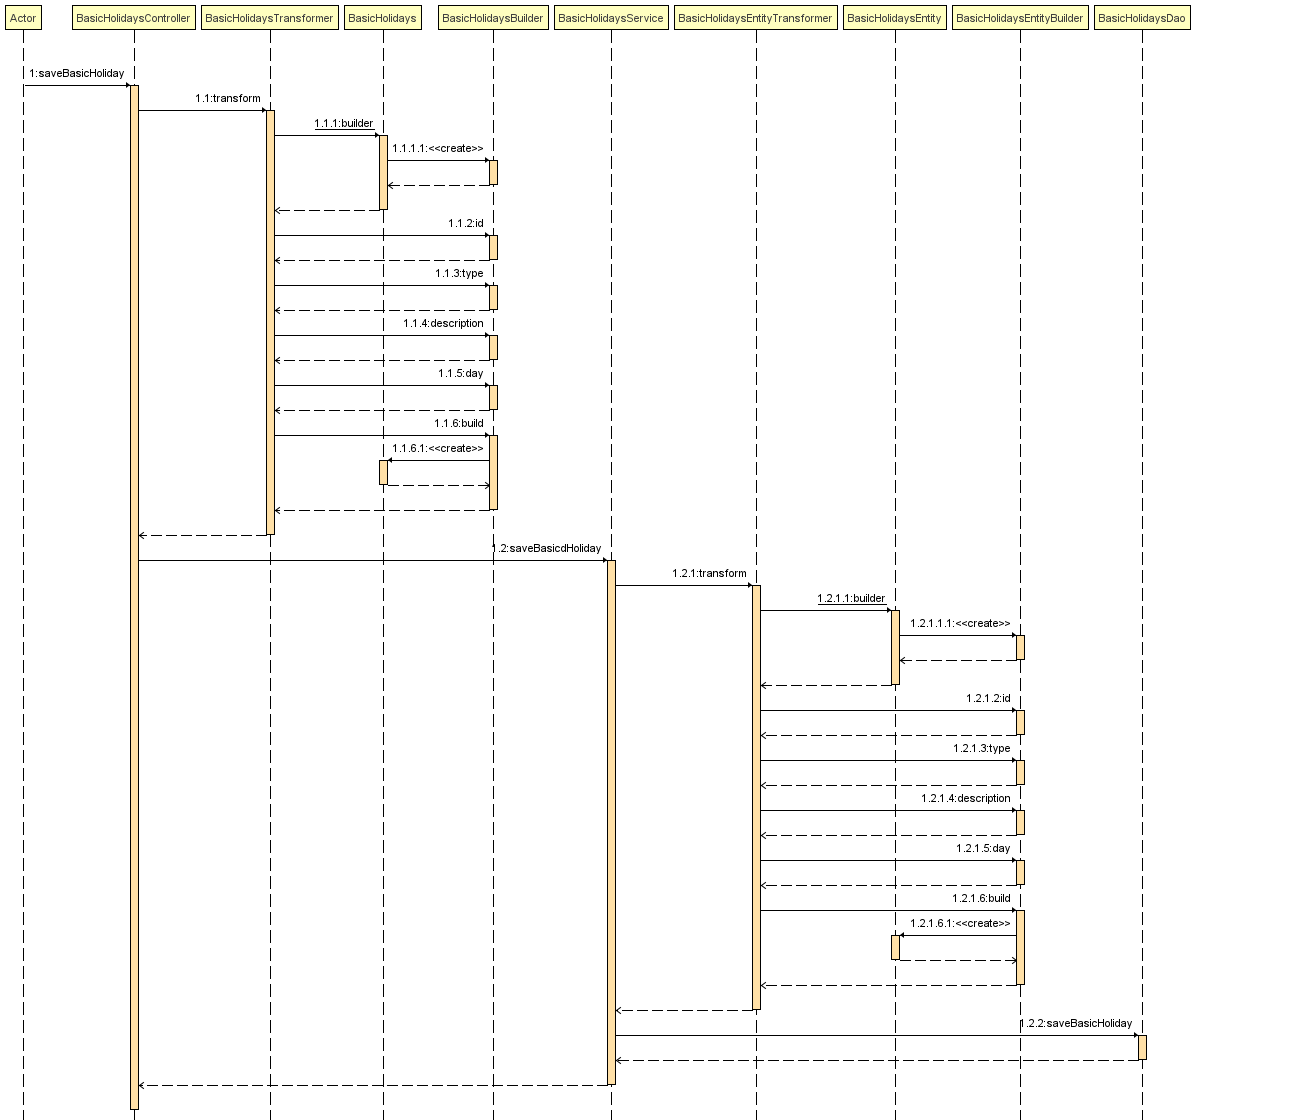
\includegraphics[scale=0.3]{images/teljesSzekvencia.png}
	\caption{HTTP Post kérés szekvenciája}
	\label{fig:teljesszekvencia}
\end{figure}

Lekérdező hívás esetén kihagyható a Belső objektumból Adatközvetítő objektumra való átalakítás, abban az esetben ha a belső objektum nem tartalmaz felesleges információt. Lényeges, hogy csak a szükséges adatokat továbbítsuk a megjelenítési réteg felé, felesleges adatok kiküldése szintén biztonsági problémát okozhat és sokkal jobban lassíthatja a megjelenítést mint a szerver oldali átalakítások. 

Az ehhez tartozó szekvenciadiagram látható \aref{fig:lekerdezoSzekvencia}. diagramon. 
\begin{figure}[h]
	\centering
	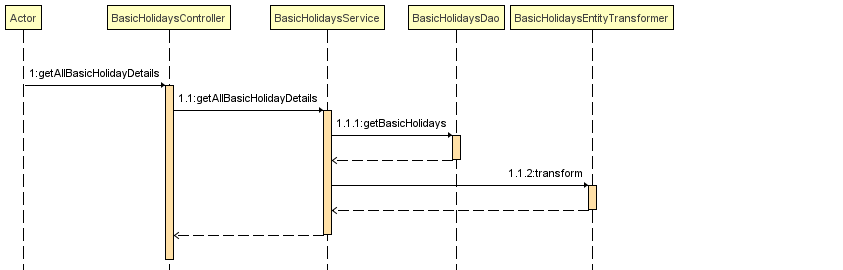
\includegraphics[scale=0.3]{images/lekérdezőSzekvencia.png}
	\caption{HTTP Get kérés szekvenciája}
	\label{fig:lekerdezoSzekvencia}
\end{figure}

Törlés esetén csak az adott elem azonosítóját várjuk paraméterként amit a gombnyomás automatikusan be tud küldeni, így validációra nincs szükség ezáltal a szekvencia is leegyszerűsödik. A törlés szekvenciája \aref{fig:törlesiSzekvencia}. diagramon látható.

\begin{figure}[h]
	\centering
	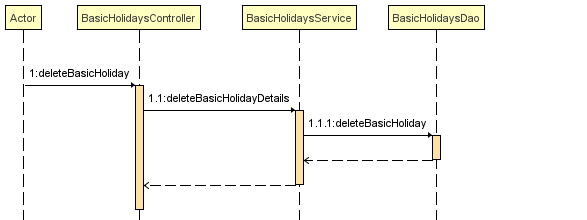
\includegraphics[scale=0.3]{images/törlésiSzekvencia.png}
	\caption{HTTP Delete kérés szekvenciája}
	\label{fig:törlesiSzekvencia}
\end{figure}

\Section{Adatbázis struktúra}
Webalkalmazások esetén az idő és erőforrás költség nagy részét az adatbázis műveleteken teszik ki, ezért fontos, hogy egyszerű és jól karbantartható struktúrát alakítsunk ki.
\vskip 0.2in
Az alkalmazáshoz tervezett adatbázis logikailag három részre bontható, kisebb önálló konfigurációs táblák,  felhasználókhoz tartozó adatok tárolása, valamint a jóváhagyási funkcióhoz szükséges táblák csoportja.

Minden logikai egység külön tervezési szemléletet igényel, ennek megfelelően az egységenkénti reláció megengedett, de az egységek közötti kapcsolatok kiépítése könnyen hibához vezethet.

\subsection{Konfigurációs táblák}

A korábban ismertetett szabadságolási szabályoknak megfelelően definiáltunk alap és pótszabadságot, valamint a pótszabadságon belül felsoroltunk több lehetőséget is, ezen lehetőségeknek saját értékeik és feltételeik vannak.

Alapvetően minden típushoz tartoznia kell egy egyedi azonosítónak és egy szám értéknek ami a szabadnapokat reprezentálja, ebből a tényből kiindulva érdemes lenne egy táblában tárolni az összes típust és megkülönböztetni azokat az egyedi értékeik alapján.

Ezzel a megoldással a következő problémák merülnek fel:
\begin{itemize}
	\item Az egyedi szabályozásokhoz saját értékek tartozhatnak, ebben az esetben komplex több oszlopos táblát kell létrehoznunk amiben kifejezetten sok null értéket tárolunk el.
	\item Minden lekérdezéskor összetett keresést kell alkalmaznunk, ha adott szabadságtípust keresünk.
	\item A tábla karbantartása komplikált feladat, ami redundanciához, és teljesítményromláshoz vezethet.
\end{itemize}

Ezáltal a tervezés során arra döntésre jutottam, hogy minden szabadság típus önálló adatbázistáblában definiálok, ahogy az \aref{fig:configurationUml}. diagramon látható. Ezáltal sok kisméretű táblát hozok létre, ezzel biztosítok jobb teljesítményt és költséghatékonyabb működést az applikációmnak ezen a területén. 

\begin{figure}[h]
	\centering
	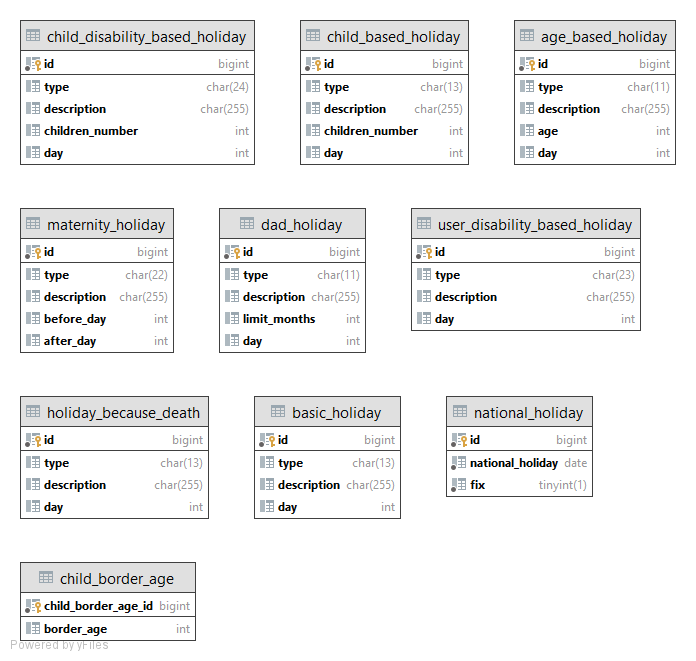
\includegraphics[scale=0.3]{images/configuration.png}
	\caption{Konfigurációs táblák UML diagramja}
	\label{fig:configurationUml}
\end{figure}

Továbbá a táblák tartalmát képezi egy típus érték is ami minden esetben konstansként jelenik meg és a pótszabadság típusát jelzi, ezzel az értékkel az automatizálási folyamat alatt megtudjuk különböztetni egymástól a típusokat.

Valamint minden tábla kapott egy leírás mezőt melyben a konfiguráció során elnevezhetjük az adott sort, hogy az egyes sorokat a felhasználó a felületen keresztül könnyebben megkülönböztesse.
\vskip 0.2in
Az időarányos szabadnapok számolásához, szükség van még a nemzeti ünnepek tárolása is, a tábla értéke megjelölhető egy boolean segítségével. \footnote{A boolean jelölés szerepét az implementáció alatt részletezem}

	Az alap szabadság esetén az adminisztrátor konfigurálhat egy 20 munkanapos szabadságot az "átlag" leírással, valamint egy 21 munkanapos sort is felvehet a "közalkalmazott" értékkel.


\subsection{Felhasználói adatok}

Az egység célja, hogy csak és kizárólag olyan adatot tároljunk a felhasználóról ami feltétlenül szükséges lesz az automatizáláshoz,mivel léteznek olyan pótszabadságok amik ha a jogszabály nem is változik maga a szabadság értéke függ a felhasználó bizonyos változó adataitól, ezért automatizálás szempontjából a változó adatokat állandó értékekből érdemes számolni a programban.

\begin{figure}[h]
	\centering
	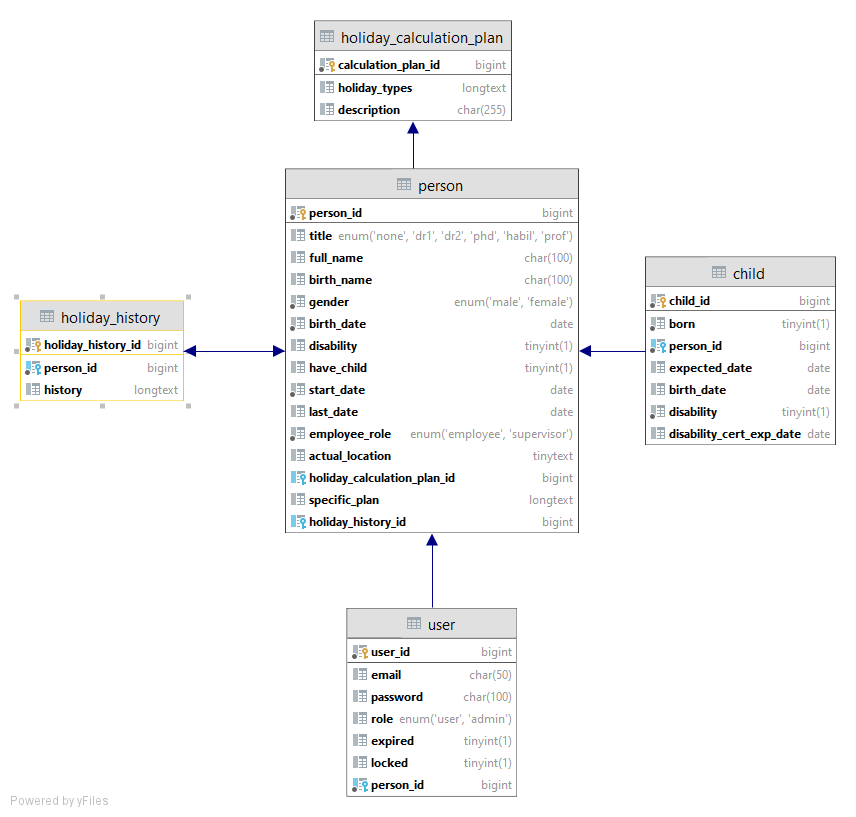
\includegraphics[scale=0.4]{images/felhasznalotablak.png}
	\caption{Felhasználóval kapcsolatos táblák UML diagramja}
	\label{fig:felhasznaloUML}
\end{figure}

A logikai egységet \aref{fig:felhasznaloUML} diagramon láthatjuk, a táblák egyéni szerepe:
\begin{itemize}
	\item \textbf{user:} A felhasználó beléptetése során az azonosítást szolgálja
	\item \textbf{person:} A felhasználó személyes adatai amik kalkulációkhoz és automatizáláshoz szükségesek.
	\item \textbf{child:} Ez a tábla egy több kapcsolatban áll a person táblával, mivel egy felhasználónak több gyermeke is lehet ennek függvényében eltérő pótszabadságokra jogosult
	\item \textbf{holiday\_calculation\_plan:} Ebben a táblában az adminisztrátor által meghatározott számítási formák vannak tárolva.\footnote{A fejezet későbbi részében részletesen kitérek rá.}, ez a tábla is egy több kapcsolatban áll a person-nel itt viszont, egy holiday\_calculation\_plan-hez tartozhat több felhasználó.
	\item \textbf{holiday\_history:} Mindenki egyéni szabadságolási története\footnote{A fejezet későbbi részében részletesen ismertetm}, éves felbontásban tárolja az egyénekre vonatkozó szabadságolási adatokat. 
\end{itemize} 
Érdemes még kitérni a "person" tábla néhány elemére:
\begin{itemize}
	\item \textbf{disability:} Pótszabadság illeti az alkalmazottat amennyiben valamilyen tartós egészségkárosodással él, mint például erőteljesen látás sérült.
	\item \textbf{have\_child:} A szülőis státusz gyors megállapítását hivatott biztosítani.
	\item \textbf{start\_date:} A munkaviszon kezdeti időpontja.
	\item \textbf{last\_date:} A munkaszerződés utolsó napja. (Opcionális érték)
	\item \textbf{employee\_role:} A felettes beosztott viszony definiálásában segít.
	\item \textbf{specific\_plan:} Az általános holiday\_calculation\_plan speciálisan a felhasználóra alakított változata.\footnote{A dolgozat későbbi részében részletesen bemutatom.}
\end{itemize}

Mindezek mellett, a "child" tábla is összetett adatokat tartalmaz:
\begin{itemize}
	\item \textbf{born:} Megmutatja, hogy a szóban forgó gyermek, megszületett-e már.
	\item \textbf{expected\_date:} A születés várható időpontja (Csak akkor létezik, ha born = false).
	\item \textbf{birth\_date:} A születési dátum, több felhasználási módja is van (Csak akkor létezik ha born = true).
	\item \textbf{disability:} Amennyiben a gyermek tartós fogyatékkal él a szülőt pótszabadság illeti.
	\item \textbf{diability\_cert\_exp\_date:} A szülő köteles bemutatni a gyermeke tartós hátrányos helyzetéről szóló határozatot, ennek egyes esetekben van lejárati ideje.
\end{itemize}
\subsection{Összetett adatok tárolása kisméretű táblákban}
Bizonyos objektumok túlságosan összetettek ahhoz, hogy ezeket egy a már bemutatott egyszerűsített adatbázisban tároljunk, amennyiben összetett egy több kapcsolattal teletűzdelt adatbázisrendszerben valósítjuk meg, az könnyedé vezethet rendkívül bonyolult struktúrát, és hosszan tartó komplex lekérdezéseket.

Megfigyelhető \aref{fig:felhasznaloUML} diagramon, hogy a \textbf{holiday\_types}, \textbf{specific\_plan}, és a \textbf{history} mezők longtext érték definíciót kaptak. Ez a tervezési döntés azért született, hogy az applikáció Belső objektumaiban bonyolult osztályhierarchiában álló adatokat egyetlen JSON-ben tudjam tárolni.

Ezzel a megoldással több tábla és több-száz sornyi adatbázis rekord létrehozását és tárolását kerülöm el, nem csak a nagy mennyiségű tárhelyet csökkentem hanem a lekérdezések bonyolultságát is, ezzel együtt az applikáció teljesítménye is növekszik.

Fontos megemlíteni, hogy ez a tervezési döntés nagyban hozzájárul az automatizálás megvalósításához, mivel az időigényes adatbázis műveletek lecsökkennek egyetlen lekérdezésre, aminek a végén a String típusú eredményből könnyen kezelhető objektum keletkezik.

\subsection{Jóváhagyáshoz szükséges táblák}
Ma a szoftverfejlesztésben gyakori igényt képez, hogy a felettesek jóváhagyják beosztottaik különböző kéréseit, ez önmagában komoly tervezést igénylő probléma, viszont megoldható egy létező ingyenes API hívással ami a saját adatbázisunkban dolgozik. A kiszolgáló legenerálja a számára szükséges táblákat és menedzseli azokat.\cite{flowable}

\Section{Funkció tervezés}

Az elvégzett igényfelmérés, és a már létező megvalósítások alapján részletesen specifikálhatóak azok a funkciók amelyek teljes megvalósítása esetén az applikáció teljesen elkészültnek minősíthető. Lényeges megemlíteni, hogy amennyiben a megvalósítás során megfelelő fontossági sorrendet tudunk állítani elérhető az a pont a fejlesztésben, ahonnan a program üzembe helyezhető. Ezzel már nagyban könnyíteni a felhasználók munkáját, amíg a további fejlesztések folynak.

Minden itt leírt funkció esetén megvalósításnál a fejezet elején lefektetett architektúra követése az elvárt működés része.

\subsection{Felhasználó és hozzáférés kezelés}

A szoftverbiztonság kiemelten fontos még a belső hálózaton működő rendszereknél is, viszont amennyiben a Webapplikációnk nyilvános címen üzemel a hozzáférés kezelés elengedhetetlen. 

A program ezzel kapcsolatos működési követelményei:
\begin{enumerate}
	\item A felhasználó egyedi felhasználónév és jelszó segítségével be tud jelentkezni a felületre, továbbá van kijelentkezési lehetősége is.
	\item Minden felhasználó csak és kizárólag a jogkörének megfelelő oldalakhoz és funkciókhoz fér hozzá.
\end{enumerate}

\paragraph{Adminisztrátor jogkör}
Többnyire az intézeti/tanszéki adminisztrátor tölti be ezt a szerepet, ehhez a jogkörhöz tartozik, a legtöbb hozzáférés és funkció.
\subparagraph{Felhasználó létrehozása}
Alapvető adminisztrátori feladat, amely során a külön erre létrehozott menüpont alatt az ügyintéző megadja a következő felhasználói adatokat:
\begin{itemize}
	\item egyedi email címe,
	\item teljes neve,
	\item jogköre.
\end{itemize}
A létrehozás gombra kattintva, a program létrehozza az adatbázisban az új felhasználót.

\subparagraph{Felhasználó adatainak lekérdezése és módosítása}
Az adminisztrátor megnyithatja az a menüpontot ahol kilistázzuk az összes alkalmazottat, a listában tud keresni, megfelelő gombra kattintva tovább navigáljuk a felhasználó részletese adatait tartalmazó oldalra, ahol a következő funkciókat tudja használni: 
\begin{itemize}
	\item felhasználói adatok szerkesztése és mentése,
	\item felhasználó gyermekeire vonatkozó adatok szerkesztése és mentése,
	\item adatok törlése,
	\item felhasználóhoz kapcsolódó szabadságra vonatkozó adatok hozzárendelése, generálása (specializált szabadság szabályzat). 
\end{itemize}

\subparagraph{Felhasználóra vonatkozó szabadságolási szabályok létrehozása}
Az adminisztrátor rendelkezik olyan funkcióval ahol menedzselhet szabadságolási szabályokat, amely tartalmazza a kiválasztott alap szabadságot, és a felhasználókra vonatkozó pótszabadságok típusainak listáját.

\paragraph{Felhasználó, felettes jogkör}
Ebben a jogkörbe tartozik a szervezeti egység vezetője, lekérdezheti az beosztottak listáját, és azok szabadság történetét.

\subparagraph{Alkalmazotti kérések bírálása}
A felettes rendelkezik olyan menüponttal, ahol lista nézetben láthatja a beosztottak szabadságolással kapcsolatos kérelmeit, azokon a következő műveleteket tudja végezni:
\begin{itemize}
	\item Kérelem elfogadása,
	\item Kérelem visszautasítása,
	\item Visszautasítás indoklása.
\end{itemize}

\subparagraph{Éves szabadságterv készítése és módosítása}
Elérhető egy felület ahol naptár nézetben jól elkülöníthető színekkel jelezve könnyen szerkeszthető és menthető az éves szabadságolási terv.

\paragraph{Felhasználó, beosztott jogkör}
A legtöbb felhasználó ebbe a jogkörbe tartozik, az általuk látható és használható funkciók a legkevesebb.

\subparagraph{Saját adatok lekérdezése}
A felhasználó bármikor lekérdezheti, de nem módosíthatja az adatokat amiket az adatbázisban tárolunk róla.

\subparagraph{Saját szabadnapok kiírása, nyomon követése}
A korábban definiált szabályoknak megfelelően képes létrehozni szabadnapokat, amelyek a felettesi bíráláson keresztül mennek, a már létrehozott szabadnapok módosítása újbóli bírálásra kerül. 

A felületen megtekintheti az éves szabadnapjainak a számát valamint a még fel nem használt napok is kijelzésre kerülnek.
\vskip 0.2in
Fontos, hogy ezek a funkciók a többi jogkörben is elérhetőek! 

\subsection{Szabadságolási szabályok konfigurálása}
Kulcsfontosságú funkció ami az adminisztrátori jogkör alá tartozik.

\paragraph{Alap és pótszabadságok}
Minden szabadságtípushoz tartozik egy egyedi, különálló felület ahol a szabályoknak megfelelően szerkeszthetőek, minden esetleges további konfiguráció jól érthető külön felületen van létrehozva.

	Alapszabadság konfigurálásához a felhasználó a következő lépéseket kell végrehajtsa:
	\begin{enumerate}
		\item Elnavigál az alapszabadságok menüpont alatt a listanézetre
		\item A hozzáadás gombra kattintva átirányítjuk az alapszabadság létrehozása űrlaphoz.
		\item A felület kitöltése után rákattint a mentés gombara.
		\item Sikeres végrehajtás esetén átirányítjuk a listanézetre, ellenkező esetben a megfelelő hibaüzenettel tájékoztatjuk.
	\end{enumerate}

\paragraph{Nemzeti ünnepek}
Ezen dátumok ismerete fontos részét képezik az éves szabadság arányos számolásának, rendkívül fontos az automatizálás szempontjából, hogy minden évben a valóságot tükrözze az általunk tárolt adat.

Az elvárt működésnek több megvalósítási lehetősége van:\footnote{A megvalósítás alatt ezekkel a lehetőségekkel részletesen foglalkozok.}
\begin{enumerate}
	\item Az adminisztrátor kézzel konfigurálja ezeket az adatokat minden évben.
	\item A manuális konfiguráció során megjelöljük a nem mozgó dátumokat amit automatikusan újra tudunk számolni, minden mást évente kézzel konfigurál a felhasználó.
	\item Az állandó dátumokat SQL segítségével beégetjük az adatbázisba, a mozgó dátumokat újraszámoljuk.
	\item Külső API hívás segítségével lekérdezzük minden év elején az adatokat amikre kíváncsiak vagyunk. 
\end{enumerate}

\subsection{Automatizált működés}
A rendelkezésre álló információk alapján az automatizálható funkciók főként az éves kalkulációkkal és tervezési munkálatokkal kapcsolatosak, ezeken felül viszont mindennapos automatizált futással a gyermekszületéssel kapcsolatos adatok alapján automatizálható az ehhez kacsolódó esemény alapú pótszabadságok kezelése is.

\paragraph{Éves szabadnapok időarányos számolása}
Ez a funkció csak részben automatizálható, amennyiben az adminisztrátor év közben hoz létre felhasználót abban az esetben biztosítanunk kell egy gombot számára amivel lehetősége nyílik az azonnali számolások elindítására.

Az automatizálással kapcsolatos műveletek a következők:
\begin{enumerate}
	\item Minden év utolsó napjának a végén a megfelelő számolást és módosítást végző funkciók futása,
	\item A felhasználóhoz rendelt szabályok, specializált formájának aktualizálása.
	\item Az aktualizált szabályok alapján az éves szabadság kiszámolása.
	\item Az éves szabadság arányos újra számolása tört év esetén.
	\item Az új éves történet létrehozása, és az éves szabadságkeret hozzáadása.
	\item Szabadság történet frissítése és mentése a megfelelő felhasználóhoz csatolva.
\end{enumerate}

\paragraph{Születéssel kapcsolatos szabadnapok esemény alapú kezelése}
Ez az automatizálás napi szintű futtatást igényel ezeket az ellenőrzéseket nap végén érdemes elvégezni.

A tervezett működés lépései a következőek\footnote{Férfiak és nők esetén a szabályozások különböznek így a megvalósításban pontosabb képet kaphatunk a témáról.}:
\begin{enumerate}
	\item Az érintett alkalmazottak kikeresése.
	\item A szabályozásnak megfelelő szabadságok létrehozása
	\item Az éves történet módosítása, és mentése.
	\item Esetleges utólagos ellenőrzések elvégzése.
\end{enumerate}

\paragraph{Éves szabadságterv generálása}
Ennek a funkciónak az automatizálása, a legösszetettebb, mivel nem csak az országos szabályozásoknak de az intézmény szabályainak is eleget kell tennünk.

Az automatizált futásnak minden év december 31. előtt meg kell történnie, a tervezett lépései:
\begin{enumerate}
	\item Az összes felhasználó lekérdezése.
	\item A felhasználók adatainak frissítése.
	\item Éves szabadság egyenlegük arányos kiszámolása.
	\item A szabadnapjaik beosztása a 7-14 napos szabálynak megfelelően.
	\item Az egyetemi szabályzatban előírtak betartása.
	\item Szabadságterv mentése egy saját adatbázis táblába.
\end{enumerate}
\subsection{Szabadságolási statisztikák készítése}
Az adminisztrátor jogkörrel rendelkező felhasználónak elérhető, egy menüpont az oldalon, ahol statisztikákat tud generálni az intézet alkalmazottainak adatai alapján.

A funkcióban a következő működések szerepelhetnek:
\begin{itemize}
	\item Statisztika kimenetének kiválasztása(diagramok, táblázatok, esetleg formanyomtatványok),
	\item Adatok intervallumának dinamikus állíthatósága,
	\item A statisztikák alanyainak beállítása.
\end{itemize}
